\documentclass{sig-alternate}
\usepackage{etoolbox}
\makeatletter
\patchcmd{\maketitle}{\@copyrightspace}{}{}{}
\makeatother

\usepackage[caption=false]{subfig}
\usepackage{verbatimbox}
\providecommand{\e}[1]{\ensuremath{\times 10^{#1}}}
\usepackage{enumitem}




\begin{document}

\title{Markov Decision Processes, Planning Algorithms, and Reinforcement Learning}
\subtitle{Writeup for Assignment 03 - CS 6741}

\author{
\alignauthor
Magahet Mendiola
}
\date{}

\maketitle
\begin{abstract}
An empirical analysis of planning and reinforcement learning algorithms in the context of Markov decision processes.
\end{abstract}

\section{Planning Metrics}
A number of simple metrics were used to evaluate the performance of our planning algorithms. These include the number of iterations and elapsed time required to find the optimal utility values for each state. However, the goal of planning is to find the optimal policy for an MDP, and not the optimal set of utility values. Therefore, we can also compare how long it takes each to find the optimal policy for each state.

There is also the rate at which a policy converges toward the optimum. This can be seen with the hamming distance between the current policy and the optimal policy at each iteration. If a partial plan can be created quickly, it may be good enough for practical use on the MDP.

Another derivation of the hamming distance metric is the time/iterations required to find the policy which will successfully guide a deterministic agent to the goal state. The idea behind this metric is that there may be many states that are never visited. Running value or policy iteration until enough of the states have optimal policies to guide the agent could greatly reduce planning time. Creating a planning algorithm with this stopping criteria would be similar to q-learning in regards to limiting exploration. It would also be similar to a* path finding, with search areas radiating omni-directionally from non-zero reward states.


\section{Grid Worlds}

Each algorithm was tested against contrived grid world type MDPs. These worlds were setup to accentuate the strengths and weaknesses of each algorithm. They also illustrate the impact of rewards, discounts, and the stochastic nature of the process on the behavior of our planning and learning algorithms. 

\subsection{Discount Grid}

This grid world, titled Discount Grid \cite{project3}, is useful for illustrating the effects of utility discounting, transition function probabilities, and state rewards on optimal policies. It includes two terminal states with positive rewards (+1 closer, +10 farther) and five negative terminal states at the bottom edge of the grid. This setup allows us to explore what set of problem and solution parameters affect the goals defined by an optimal policy.

Figure~\ref{discount-default} shows the resulting values of the MDP after running value iteration with a $\gamma$ of 0.9 and a reward of 0 in all the non-terminal states. The transition probabilities are 0.8 for desired action and a combined 0.2 for all orthogonal movements. In this case, the policy directs the agent to seek out the farther, higher valued, terminal state. It also avoids the high penalty cliff except when the alternative is moving into the lower reward terminal state.

\begin{figure}[!htbp]
    \centering
    \subfloat[0.9]{\includegraphics[width=1.5in]{images/discount/default.pdf}\label{discount-default}}~
    \subfloat[0.99]{\includegraphics[width=1.5in]{images/discount/g-099.pdf}\label{discount-g099}}
    \caption{discount grid - various $\gamma$ settings}
\end{figure} 

\paragraph{Time matters}

With a $\gamma$ of 0.99, which reduces the effects of discounting, the policy shifts slightly (Figure~\ref{discount-g099}). The policy in state (2,2) now risks a direct movement to the east, given the higher expected utility of that action. This is due to the higher relative value of state (1,2) due to the reduced discounting. Also, state (3,6) avoids the risk of falling into the lower reward for the same reason. The expected value of attempting a northward movement is now relatively more valuable than with a move east policy, despite the indirect route to the terminal state. This shows the implications of adjusting delayed reward and how an agent could be lead to take greater risks or follow an otherwise sub-optimal route to gain a larger reward farther in the distance.

\paragraph{Rewards matter}

With a shift in rewards, we can affect how the resulting policy directs the agent. Figure~\ref{discount-r2} shows the result of changing the reward in all non-terminal states to -2. The policy now believes that the closer terminal state is a better alternative at state (3,2). The negative rewards, and risk of falling off the cliff, push the agent toward the closer end point. With the non-terminal rewards set to -3, this early termination policy extends to the northern path as well (Figure~\ref{discount-r3}). With a sufficiently negative non-terminal reward, we can even entice the agent to end the process as quickly as possible, by intentionally jumping off the cliff (Figure~\ref{discount-r11}).

\begin{figure}[!htbp]
    \centering
    \subfloat[-2]{\includegraphics[width=1.5in]{images/discount/r-2.pdf}\label{discount-r2}}~
    \subfloat[-3]{\includegraphics[width=1.5in]{images/discount/r-3.pdf}\label{discount-r3}}\\
    \subfloat[-11]{\includegraphics[width=1.5in]{images/discount/r-11.pdf}\label{discount-r11}}
    \caption{discount grid - various non-terminal reward settings}
\end{figure} 

\paragraph{The problem matters}

Policies are not only affected by planning algorithm parameters, but also by the problem definition, such as the probabilities in the transition function. If movement in the MDP is deterministic, or the intentional action probabilities are sufficiently high, otherwise risky paths would be considered optimal. Figure~\ref{discount-n001} shows a policy of cliff-walking given only a 1\% change of falling off the ledge. Conversely, the policy in Figure~\ref{discount-n04} shows how our planning algorithm would approach a high risk environment (inebriated agent). In the later case, the agent will avoid any east-west movement, even at the expense of exiting at the low reward terminal state.

\begin{figure}[!htbp]
    \centering
    \subfloat[0.01]{\includegraphics[width=1.5in]{images/discount/n-001.pdf}\label{discount-n001}}~
    \subfloat[0.4]{\includegraphics[width=1.5in]{images/discount/n-04.pdf}\label{discount-n04}}\\
    \caption{discount grid - various unintentional movement probabilities}
\end{figure} 


\subsection{Tunnel Grid}

Tunnel grid is a one dimensional grid with the starting state on one end and the only terminal state on the other. Although this grid is simplistic, it highlights the distinctions between our planning and learning algorithms well.

\begin{figure}[!htbp]
    \centering
    \subfloat[value iteration]{\includegraphics[width=3in]{images/tunnel/value.pdf}\label{tunnel-value}}\\
    \subfloat[policy iteration]{\includegraphics[width=3in]{images/tunnel/policy.pdf}\label{tunnel-policy}}\\
    \subfloat[q-learning]{\includegraphics[width=3in]{images/tunnel/q.pdf}\label{tunnel-q}}
    \caption{tunnel grid}
\end{figure} 

For example, Figure~\ref{tunnel-performance} shows the elapsed time and the number of iterations/episodes each algorithm took to converge. In the case of Q-learning, an episode is determined as a single training run from the starting state until the agent reaches a terminal state. Also, convergence for the Q-learning agent is defined as the state when setting $\epsilon$ to zero and following the best q-score at each state would result in the optimal policy.


\begin{table}[!htbp]
\begin{tabular}{lllll}
           & Elapsed Time & Iterations/Episodes &  &  \\
Value      & 0.04         & 29                  &  &  \\
Policy     & 0.04         & 19                  &  &  \\
Q-Learning & 0.390        & 18                  &  & 
\end{tabular}
\caption{tunnel grid - performance\label{tunnel-performance}}
\end{table}

We see from the first two rows that value iteration requires nearly 50\% more training cycles to converge. However, policy iteration and value iteration are identical in terms of elapsed time. This is due to the greater computational requirements of policy evaluation at each interval for policy iteration. Q-learning required a substantially longer amount of time to train.

In the case of the tunnel grid, Q-learning will perform identically to an agent that guesses randomly (random walk) until it eventual reaches a non-zero reward state. Until then, none of the states it visits will produce a meaningful Q-value. This is highly inefficient, as the expected number of states the agent will visit before reaching the end is $n^2 + n$ with n being the number of states between the start and terminal point. Once this state is eventually reached, the Q-values will be updated only for that state. The agent would have to return to that state again for the Q-value to propagate further. In total, the expected number of steps the agent would have to move before a full path is created in this MDP is the summation of expected values from 1 to n random walks. In a 19 state tunnel grid world, that comes out to around 3,000 expected steps before a full path of q-values are propagated.

A more intelligent agent would keep track of previously visited states that resulted in all zero q-scores and place greater action probability on moving to previously unexplored states. Another enhancement would be to remember the path taken by the agent and update q-values for the entire path once a non-zero reward state is encountered, rather than only updating the closest state.

If the grid world is modified slightly, the strengths of Q-learning become evident. With the starting state on the north wall of the tunnel and the terminal state on the south wall, the Q-learning agent does not need to randomly explore very far before finding the terminal state for the first time. In fact, it takes only three episodes and 141 total agent moves (0.01 sec) to discover the optimal path (Figure~\ref{side-tunnel-q}). If the agent was allowed to continue running, it would eventually discover the entire MDP and assign Q-scores and policies. However, there is no need. The majority of the states are superfluous and exploring them would not improve the agent's optimal path in the context of this MDP.

Figure~\ref{side-tunnel-value} shows the comparative waste with value iteration. It does a comprehensive evaluation of all the states and stops only when the furthest state update falls below the stopping threshold. It's analogous to searching an entire house before trusting that the front door will get you outside. Domain knowledge would be very helpful is guiding such algorithms. For example, the stopping condition for value or policy iteration could be set such that it triggers once a path is revealed between predetermined states. Taking this further, each of these algorithms could be modified to behave directionally; only propagating value/policy towards a target state. This would tailor them more toward the specific use case of path finding, but should work well in the context of grid worlds. It does, however, suppose special knowledge of the MDP regarding a known target state. As we saw in the discount grid example, there are many situations where the environmental conditions will dictate what should be considered the target state.


\begin{figure}[!htbp]
    \centering
    \subfloat[value iteration - 0.11 sec]{\includegraphics[width=3in]{images/side-tunnel/value.pdf}\label{side-tunnel-value}}\\
    \subfloat[q-learning - 0.01 sec]{\includegraphics[width=3in]{images/side-tunnel/q-q.pdf}\label{side-tunnel-q}}\\
    \caption{side tunnel grid}
\end{figure} 


\subsection{Simple Grid}

To evaluate value and policy iteration performance empirically as the number of states increase, each algorithm was run to convergence on grids ranging from 3 by 3 (9 states) to 30 by 30 (900 states). A single, positive valued, terminal state was set at one corner. Figure~/ref{simple-planning-performance} shows the results of this experiment. Within these grid sizes, iterations seem to grow linearly with respect to the grid edge size, which seems reasonable considering the radiating propagation behavior seen with these algorithms. Elapsed time for each shows greater than linear growth, which can be partially attributed to the polynomial growth of the number of states. Relatively, policy iteration elapsed time seems to grow at a greater rate than value iteration. At 900 states, the difference is as great as 40\% slower.


\begin{figure}[!htbp]
    \centering
    \includegraphics[width=3in]{images/simple/planning-performance.pdf}
    \caption{planning performance by grid size \label{simple-planning-performance}}
\end{figure} 

Hamming distance over time is shown in Figure~\ref{simple-hd}. This plot shows how each algorithm converges toward an optimal policy. Policy iteration, although slower overall, shows a smooth transition as it updates the policy at each adjacent state during subsequent iterations of the algorithm. Value iteration updates may not update state policies each time, and we see from the plot that with around 300 non-optimal state polices, the performance curve makes a significant behavioral shift. This is probably due to change in the time complexity of updating each state as non-zero values are propagated outward from the terminal state. The policy iteration curve likely smooths the effects of these state value updates over the entire curve, as fully converged values are assigned to each state during every iteration.

\begin{figure}[!htbp]
    \centering
    \includegraphics[width=3in]{images/simple/hd.pdf}
    \caption{algorithm convergence over time \label{simple-hd}}
\end{figure} 


\subsection{Random Grid}

Theoretically, performance of both value and policy iteration are determined by the number of states and actions. To validate this empirically, an experiment was conducted which generates random grid worlds of a fixed size. A random number of positive and negative terminal states were scattered throughout the grid, along with a random number of unreachable states. Figure~\ref{random} shows an example of one of these grid worlds. Value and policy iteration was performed on each of these grids to determine if iteration or time performance would vary with each layout. Through thousands of such random generations, performance was almost identical between each planning process. The only variance being accounted for by random isolated states (surrounded by walls).

\begin{figure}[!htbp]
    \centering
    \includegraphics[width=3in]{images/random.pdf}
    \caption{random grid \label{random}}
\end{figure} 

Q-learning on these random grids performed with mixed results, depending on the starting state of the agent. In some cases, the agent was restricted to an isolated section of the grid by walls. In these cases, exploration of the reachable area was completed quickly and an optimal policy was discovered to the nearest positive terminal state. Performance was also affected by the general shape of the grid. As we noted with the tunnel grid example, Q-learning performed well when positive terminal states were close to the starting state and larges sections of the grid could essentially be ignored. In these situations, stopping criteria would be helpful. Something similar to the update threshold in value and approximate policy iteration. In fact, a reverse of epsilon greedy search could work well. The process would involve decreasing epsilon until an established path was determined. Epsilon would then be increase to encourage the agent to focus on exploration. Given that that optimal policy is already determined, there is less need for improving the already established path and more effort can go into finding alternative paths and reward states.


\section{Value Iteration}


\section{Policy Iteration}

\section{Q-Learning}

metrics
    elapsed time
    hamming distance

lazy vs. eager learning.

planning performance

policy iteration implementation issues
    get's stuck with only policy change check
    takes too long with epsilon check
    works well with value update check


q-learning performnace
q-learning strategies








\bibliographystyle{abbrv}
\bibliography{references}


\end{document}
